\chapter{Teori og tidligere arbeid}
\label{kap:teori}

\section{Teori}
Rotårsaksanalyse er en måtefor å finne roten til et problem. Måten den finner roten er ved å analysere de underliggende faktorene og bruker de til å finne roten til problemet. RCA er en unik reaktiv prosess som finner svar basert på skjulte årsaker og deres effekt enn å bare se på den mest åpenbare årsaken. Det gjør at finne rotårsaken er ofte komplekst og tidkrevende, men når rotårsaken først er funnet vil løsningen eller løsningene bli relativt åpenbare.    
    \subsection{Historie}
    Det har finnes flere varianter av rotåsaksanalyse opp gjennom tidene, men mannen som er kreditert med å finne opp rotårsaksanalyse er grunnleggeren av Toyota, Sakichi Toyoda. Hans versjon av RCA ble tatt i bruk av Toyota produksjons prosess i 1958 og ble kalt "5 Whys". Som tidligere sagt har RCA forandret seg over tidene for å imøtekomme de forskjellige feltene, så nå brukes RCA som verktøy i flere felter som transport, medisin og luftfart. 
    
    \subsection{Ulike nivåer av årsaker}
    Et problem er som regel ikke et resultat av en årsak, men heller en kombinasjon av flere årsaker på flere forskjellige nivå. Dette vil si at årsaker påvirker andre årsaker og det igjen blir det synlige problemet. Vi kan definere årsaker i tre forskjellige grupper.
    \begin{description}
    \item[Symptomer] er ikke å regne som faktiske årsaker, men heller bevis på eksisterende problemmer.
    \item[Første-nivå årsak] er årsåker som leder direkte til et problem.
    \item[Høy-nivå årsaker] er årsåker som blir til første-nivå årsaker. Selv om de ikke direkte er årsak til problemmet, skaper høy-nivå årsak lenker i kjeden av årsak og effekt forholdet som til slutt fører til problemet.  Den høyeste nivå årsaken er rotårsaken.  
    \end{description}
Noen problemer har flere årsaker som er forbundet av de forskjellige faktorer som kombinert blir til problemet.

\begin{figure}[H]
    \centering
    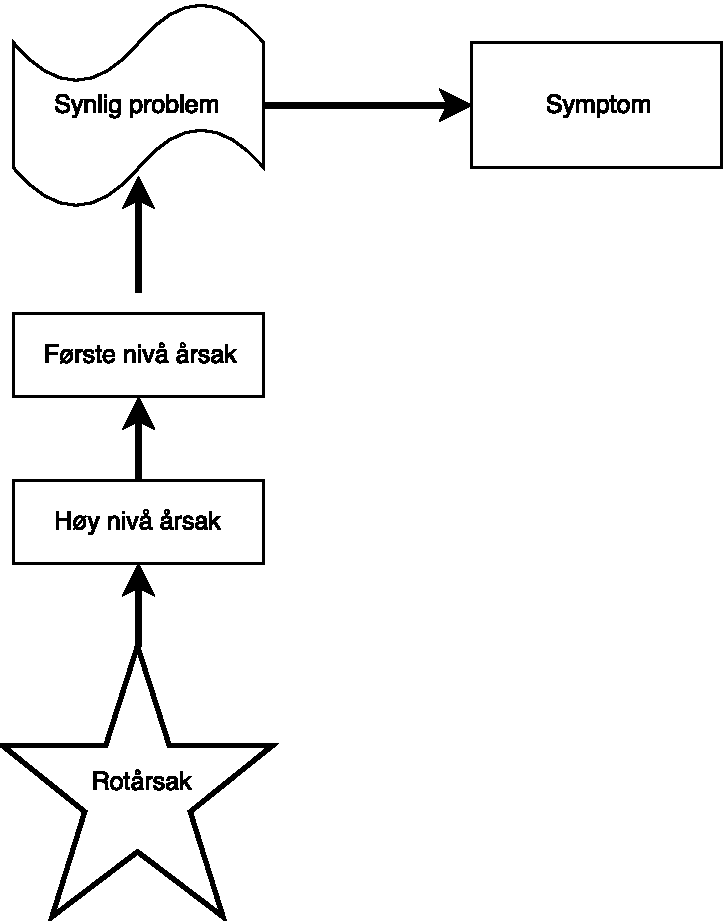
\includegraphics[scale=0.6]{main/bilder/nivaa.pdf}
    \caption[Nivå]{De forskjellige nivåer til problemet}
    \label{fig:nivaa}
\end{figure}

Vi ser fra figuren at rotårsaken er det som setter igang hele årsak og effekt kjeden som leder til problemet. 

    \subsection{Rotårsaksanalyse mot risikoanalyse}
    En risikoanalyse ser på sannsynlighet for at en trussel kan skje og hva mulige konsekvenser vil være. Risikoanalysen vil bruke dataene fra sannsynlighet- og konsekvensvurderingen til å finne mulige preventive og reaktive tiltak som vil brukes til å få riskoen ned på et akseptabelt nivå. Rotårsaksanalyse vil på sin side gjøre en systematisk gjenomgang for å finne de underliggende årsakene til feil eller svikt. En rotårsaksanalyse gjøre etter en hendelse har inntruffet, i motsetning til riskoanalyse som gjøre for å behandle fremtidlige situasjoner.    
\section{Tidligere arbeid}
 I 2016 ga NTNU en bacheloroppgave som brukte rotårsaksanalyse på tre forskjellige caser. Oppgaven viste at rotårsakanalyse fungerer i en informasjonsikkerhet sammenheng. Vår oppgave skal jobbe videre med å se på hvordan rotårsaksanalyse fungerer i informasjonsikkerhet.    

